% Garis istimewa segitiga dengan TikZ: garis tinggi, garis berat, garis bagi.
% Segitiga yang sama dipakai di ketiga gambar: A(0,0), B(6,0), C(2,4).
% Kompilasi: pdflatex garis-istimewa-segitiga.tex (butuh paket tikz).
\documentclass{article}
\usepackage{tikz}
\usetikzlibrary{calc}
\begin{document}

% ---------------- Gambar 1: garis tinggi dari C ----------------
\begin{figure}[h]
\centering
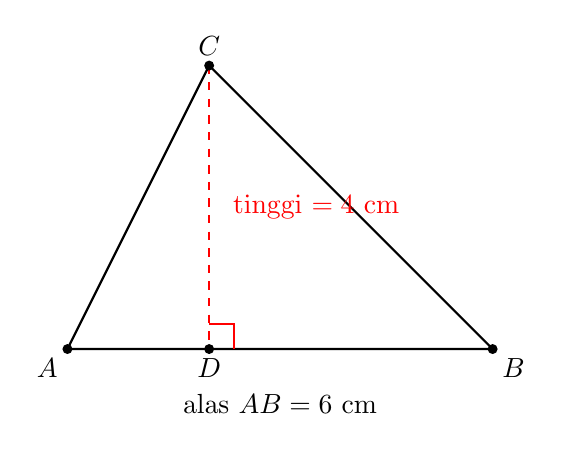
\begin{tikzpicture}[scale=0.9]
  \coordinate (A) at (0,0);
  \coordinate (B) at (6,0);
  \coordinate (C) at (2,4);
  \coordinate (D) at (2,0); % kaki tinggi dari C
  \draw[thick] (A) -- (B) -- (C) -- cycle;
  \draw[dashed, red, thick] (C) -- (D);
  % tanda siku di D
  \draw[red, thick] (D) ++(0.35,0) -- ++(0,0.35) -- ++(-0.35,0);
  \foreach \p/\pos in {A/below left, B/below right, C/above, D/below} {
    \fill (\p) circle (2pt);
    \node[\pos] at (\p) {$\p$};
  }
  \node[red, right] at (2.2,2) {tinggi $= 4$ cm};
  \node[below] at (3,-0.5) {alas $AB = 6$ cm};
\end{tikzpicture}
\caption{Garis tinggi dari $C$: tegak lurus terhadap alas $AB$.}
\end{figure}

% ---------------- Gambar 2: garis berat dari A ----------------
\begin{figure}[h]
\centering
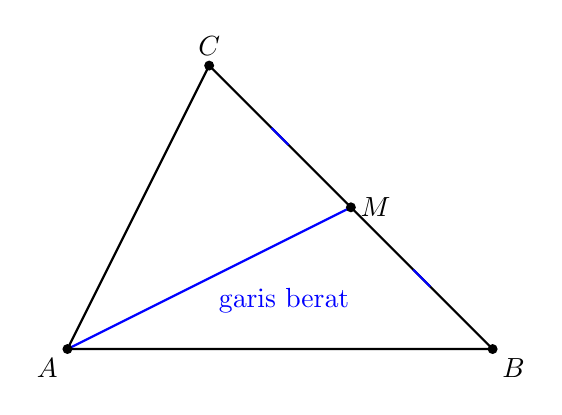
\begin{tikzpicture}[scale=0.9]
  \coordinate (A) at (0,0);
  \coordinate (B) at (6,0);
  \coordinate (C) at (2,4);
  \coordinate (M) at ($(B)!0.5!(C)$); % titik tengah BC = (4,2)
  \draw[thick] (A) -- (B) -- (C) -- cycle;
  \draw[blue, thick] (A) -- (M);
  % tanda sama panjang pada kedua potongan BC
  \draw[blue, thick] (5,1) ++(-0.12,0.12) -- ++(0.24,-0.24);
  \draw[blue, thick] (3,3) ++(-0.12,0.12) -- ++(0.24,-0.24);
  \foreach \p/\pos in {A/below left, B/below right, C/above, M/right} {
    \fill (\p) circle (2pt);
    \node[\pos] at (\p) {$\p$};
  }
  \node[blue, below right] at (2,1) {garis berat};
\end{tikzpicture}
\caption{Garis berat dari $A$: menuju titik tengah $M$ sisi $BC$.}
\end{figure}

% ---------------- Gambar 3: garis bagi sudut A ----------------
\begin{figure}[h]
\centering
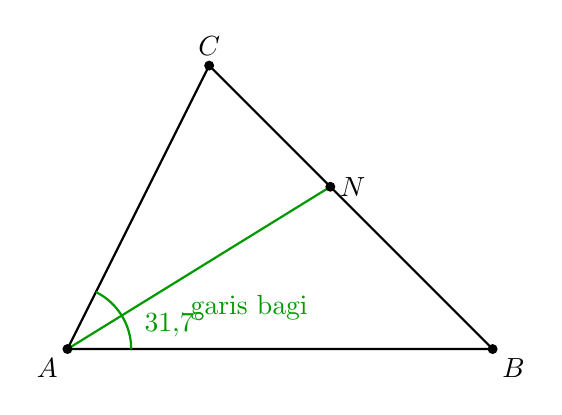
\begin{tikzpicture}[scale=0.9]
  \coordinate (A) at (0,0);
  \coordinate (B) at (6,0);
  \coordinate (C) at (2,4);
  % titik bagi pada BC: AB : AC = 6 : 4,47
  \coordinate (N) at (3.71,2.29);
  \draw[thick] (A) -- (B) -- (C) -- cycle;
  \draw[green!60!black, thick] (A) -- (N);
  % busur sudut A (63,4 derajat), dibelah garis bagi menjadi 31,7 + 31,7
  \draw[green!60!black, thick] (A) ++(0.9,0) arc (0:63.4:0.9);
  \foreach \p/\pos in {A/below left, B/below right, C/above, N/right} {
    \fill (\p) circle (2pt);
    \node[\pos] at (\p) {$\p$};
  }
  \node[green!60!black, below right] at (1.6,0.9) {garis bagi};
  \node[green!60!black, right] at (0.95,0.35) {$31{,}7^\circ$};
\end{tikzpicture}
\caption{Garis bagi sudut $A$: membagi $63{,}4^\circ$ menjadi $31{,}7^\circ + 31{,}7^\circ$.}
\end{figure}

\end{document}
